\chapter{OpenAI Gym and Universe}
\label{chapter4}

\begin{quotation}
    {\footnotesize
    \begin{flushright}
    \noindent{\emph{\textbf{Hinton} set the baseline for neural networks \\
    \textbf{LeCun} set the baseline for convolutional neural networks \\
    \textbf{ImageNet} set the baseline for visual recognition competitions \\
    \textbf{DeepMind} set the baseline for deep RL algorithms \\
    \textbf{OpenAI} set the baseline for deep RL environments}}
    \end{flushright}}
\end{quotation}

\vspace{0.5cm}

\noindent After all the initial chapters regarding the reinforcement learning theory, it is a must to introduce \textbf{openAI} that, as written on their website~\cite{openAI}, \textit{is a non-profit AI research company, discovering and enacting the path to safe
artificial general intelligence}.

OpenAI has published many works, especially in reinforcement learning, and has released two main tools to improve and forward research and publication in this field. \\
The two main tools are \textbf{Gym}~\cite{gym}, a toolkit for developing and comparing reinforcement learning algorithms and \textbf{Universe}, a software platform for measuring and training an AI’s general intelligence across the world’s supply of games, websites and other applications.

For this project, the Universe environment of \textbf{Atari Pong} has been used, one of the first ever commercialized games, together with the \textbf{Universe Starter Agent}, a learning environment developed by openAI and available in their github repository~\cite{universe-starter-agent}.
\begin{figure}
    \centering
    \includegraphics[width=0.6\textwidth]{./pictures/universe.eps}
    \caption{Some of the environments available in Universe.}
    \label{fig:universe}
\end{figure}

\section{Starter Agent}
Universe Starter Agent is the implementation of the A3C~\cite{a3c} algorithm adapted for Atari games and Universe environments. This implementation allows the utilization of all the environments available in Universe simply by specifying the interested one from command line.

In this implementation, the policy is estimated through a long short term memory (LSTM) network with 256 hidden states.
\newline
\newline
\noindent
The command to start the agent is:
\begin{lstlisting}[frame=single]
python train.py --num-workers 2
    --env-id PongDeterministic-v3 --log-dir /tmp/pong
    --visualise
\end{lstlisting}
where \texttt{--num-workers} is the number of threads spawned by the command, each one running its own policy, \texttt{--env-id} sets the environment, \texttt{--log-dir} sets the folder where to save the TensorBoard~\cite{tensorflow} files and \texttt{--visualise} is an optional parameter to view the agent playing the game in a docker screen.

When this command is executed, a new tmux session is launched with $n~+~3$ terminals where $n$ is the number of parallel agents. The 3 more terminals are dedicated to TensorBoard (one) and to check interactively the processes (two).

\section{Pong}
\begin{figure}
    \centering
    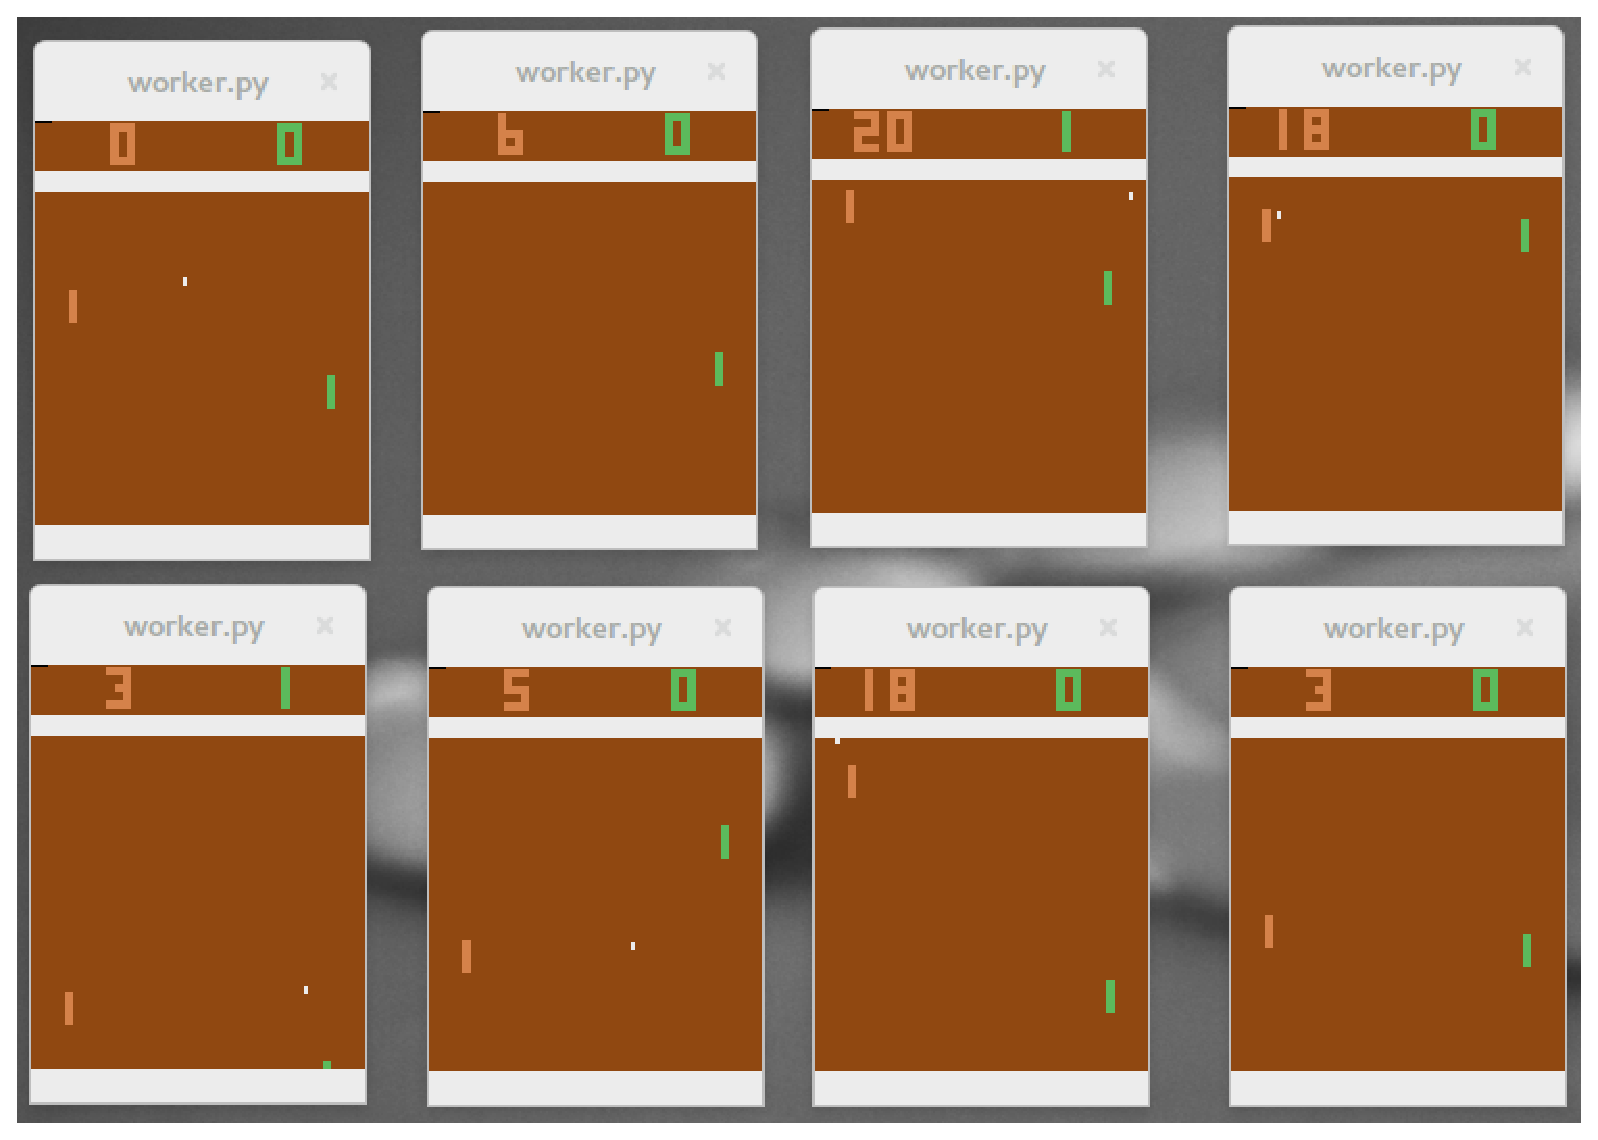
\includegraphics[width=0.6\textwidth]{./pictures/pong.eps}
    \caption{Atari Pong being played by 8 agents in parallel.}
    \label{fig:pong}
\end{figure}
Atari Pong is one of the most simple games where the two players have to move a board in order to catch the ball and send it back to the other player. A point is made when you manage to get the ball over the opponent's board. A game finishes when a player reaches 20 points.

At the beginning, I made  a test with the \textit{universe-starter-agent} default parameters and obtained, obviously, incredible results:
\begin{itemize}
    \item as expected, initially the policy was random and the agent was continuously losing the game since it didn't know what to do (the board was not moving at all);
    \item as time went by, the agent managed to move the board and catching the ball but still losing the game;
    \item it later understood that bumping the ball on one of the borders would make the ball bounce on the opposite direction making it harder for the opponent to catch it;
    \item after a sensible amount of iterations and almost 15 hours of training, each one of the 8 spawned agents was trying to make the same winning move at each step, managing to win every time with a score of 20-0.
\end{itemize}
\noindent
The 2 main hyper-parameters that can be easily modified in the code are:
\begin{itemize}
    \item the number of hidden layers in the LSTM policy estimator, default set to 256;
    \item \texttt{num\_local\_steps} which represents the amount of steps that each thread performs on its own before having policy and value functions updated. By default, this parameter is set to 20 steps.
\end{itemize}
\noindent
I decided to perform various tests changing the second parameter, the essential one in an \textit{asynchronous} algorithm.

The results were the following~\cite{universe-starter-agent}:
\begin{itemize}
    \item increasing the number of local steps lowers the variance in the estimation;
    \item increasing the number of local steps, will perform less frequent parameter updates slowing down the learning;
    \item decreasing the number of local steps below 20 makes the algorithm unable to learn.
\end{itemize}

\begin{figure}[ht]
    \begin{minipage}[b]{0.49\textwidth}
    \centering
    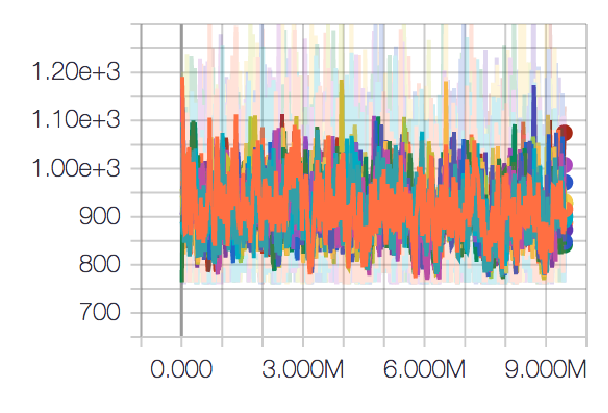
\includegraphics[width=0.99\textwidth]{pictures/5_length.eps}
    \label{fig:length5}
    \end{minipage}
    \begin{minipage}[b]{0.49\textwidth}
    \centering
    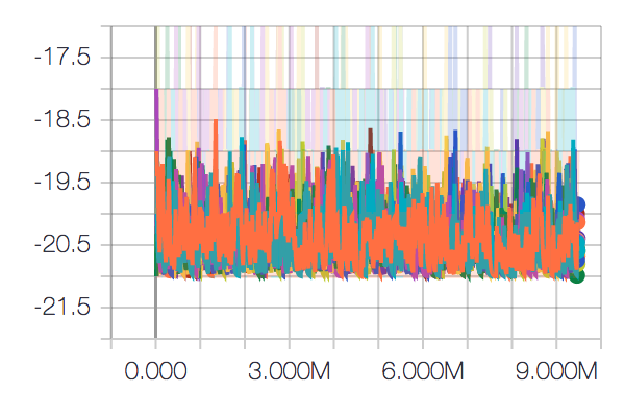
\includegraphics[width=0.99\textwidth]{pictures/5_reward.eps}
    \label{fig:reward5}
    \end{minipage}
    
    
    \begin{minipage}[b]{0.49\textwidth}
    \centering
    \includegraphics[width=0.99\textwidth]{pictures/20_length.eps}
    \label{fig:length20}
    \end{minipage}
    \begin{minipage}[b]{0.49\textwidth}
    \centering
    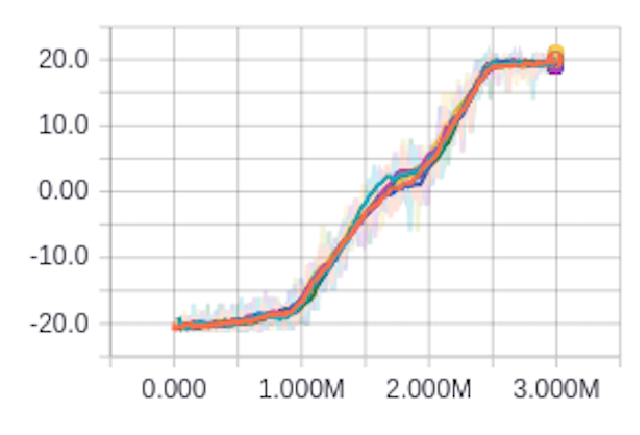
\includegraphics[width=0.99\textwidth]{pictures/20_reward.eps}
    \label{fig:reward20}
    \end{minipage}
    
    
    \begin{minipage}[b]{0.49\textwidth}
    \centering
    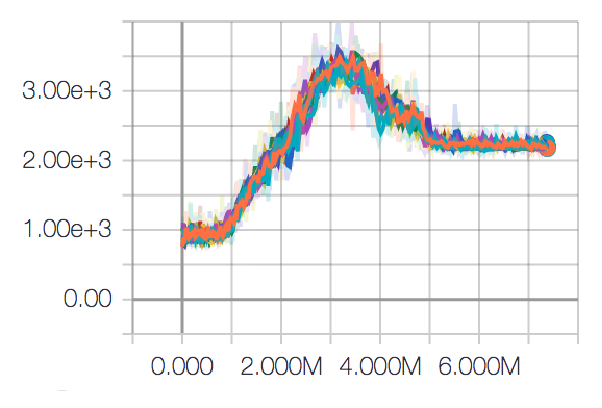
\includegraphics[width=0.99\textwidth]{pictures/50_length.eps}
    \label{fig:length50}
    \end{minipage}
    \begin{minipage}[b]{0.49\textwidth}
    \centering
    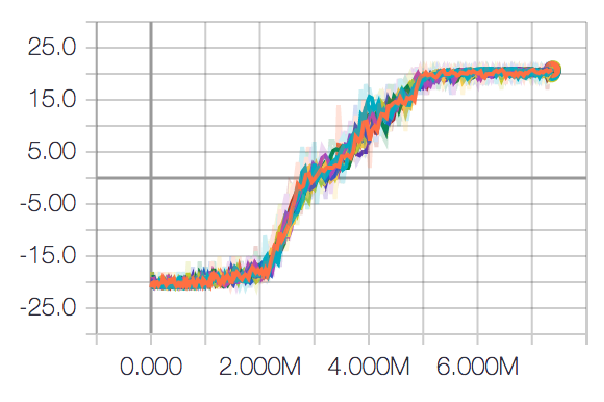
\includegraphics[width=0.99\textwidth]{pictures/50_reward.eps}
    \label{fig:reward50}
    \end{minipage}
    \caption{Above are shown the results for \texttt{num\_local\_steps} $=$ 5, first row, 20, second row, 50, third row. The first plot in each row represents the episode length while the second represents the reward per episode.}
\end{figure}